\chapter{Results}
\label{capitolo4}

This Chapter contain a first part in which the program is tested with the state of art, in order to demonstrate the correct working of the library. And, secondly, is done a deeply study of the Montel system using the implementing codes of the library.
\vspace{0.5cm}
\section{Testing}
To demonstrate the correct behaviour of the program there are done a comparison  with respect to the OASYS software for ray tracing simulation, developed by Manuel Sanchez Del Rio, and with respect to the  paper \cite{resta2015nested}. The comparison with OASYS check the correct working of all the component apart from Montel system (mirrors, lens, KB ...), on the contrary, the paper is dedicate for the Montel simulation, because this particular kind of optical system, is not implemented on OASYS.
%
\subsection{Testing with OASYS}
%
OASYS (OrAnge SYnchrotron Suite) is a graphical environment for optic simulation used in synchrotron facilities based on orange 3, developped by Manuel Sanchez Del Rio (ESRF) and Luca Rebuffi (ELETTRA).
The comparison between the program and the OASYS software is done with the system in Figure \ref{fig: Optical system}, where the 1st optical system collimate the source, the 2nd optical system focalize the mean at the image plane, the system between the source and the 1st optical system correspond to the focal distance of the system $d_1 = f = 0.4 m $, between the 12st and the 2nd optical system with a distance $d_2 = 0.6 m $ and the distance between the 2nd system and the image plane correspond to the focal length of the 2nd optical system that is $d_3 = f = 0.4$. A system that have parameters defined as before, make a copy of the source image at the image plane.
%
\begin{figure}[]
%
\centering
%
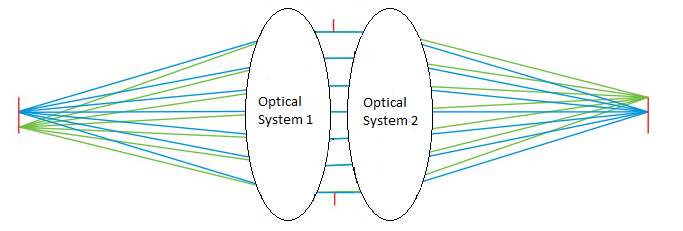
\includegraphics[width=.6\textwidth]{Immagini/Chapter4/OpticalSystems}
%
\caption{Optical system}
%
\label{fig: Optical system}
%
\end{figure}
%
The source parameter used are showed in Figure \ref{fig: Source Parameter for OASYS}, and correspond to  a square source spot of $1 \mu m^2 $, and a initial Gaussian divergence with a FWHM of $1 mrad $.
\begin{figure}[]
%
\centering
%
\subfloat[][Initial spot size \label{fig: Source OASYS}]
   {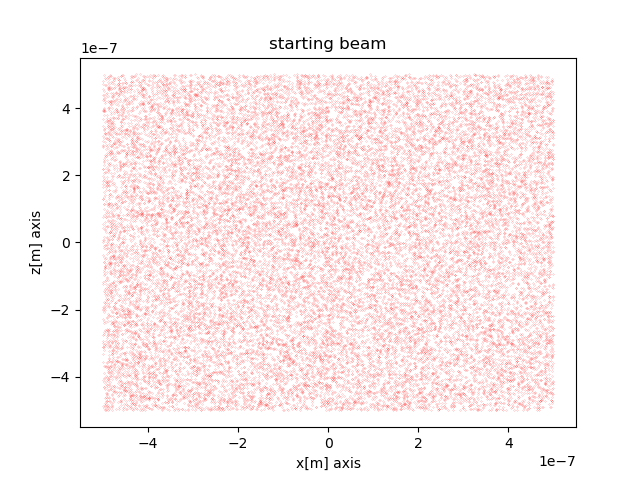
\includegraphics[width=.4\textwidth]{Immagini/Chapter4/SouceOASYS}}
%
\subfloat[][Initial Beam divergence\label{fig: Divergence OASYS}]
   {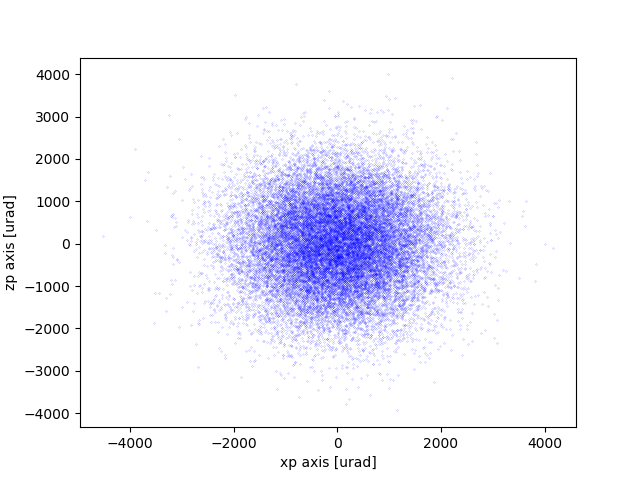
\includegraphics[width=.48\textwidth]{Immagini/Chapter4/DivergenceOASYS}}
%
\caption{Parameter of the source used for the comparison with OASYS}
%
\label{fig: Source Parameter for OASYS}
%
\end{figure}
%
The tests are done using different optical system, with the same focal length and, for the mirror it is used a grazing incidence angle of $\theta = 1.719^{\circ}$. Below are plotted the image of the Beam at the image plane, putting the OASYS' results on the right, and my results on the left. The system simulated are done with:
\begin{enumerate}
\item ideal lenses Figure \ref{fig: Ideal lense OASYS}
\item parabolic mirror Figure \ref{fig: paraboloid OASYS}
\item KB system Figure \ref{fig: KB system OASYS}
\end{enumerate} 
%
\begin{figure}[]
%
\centering
%
\subfloat[][Initial spot size \label{fig: my Ideal Lenses}]
   {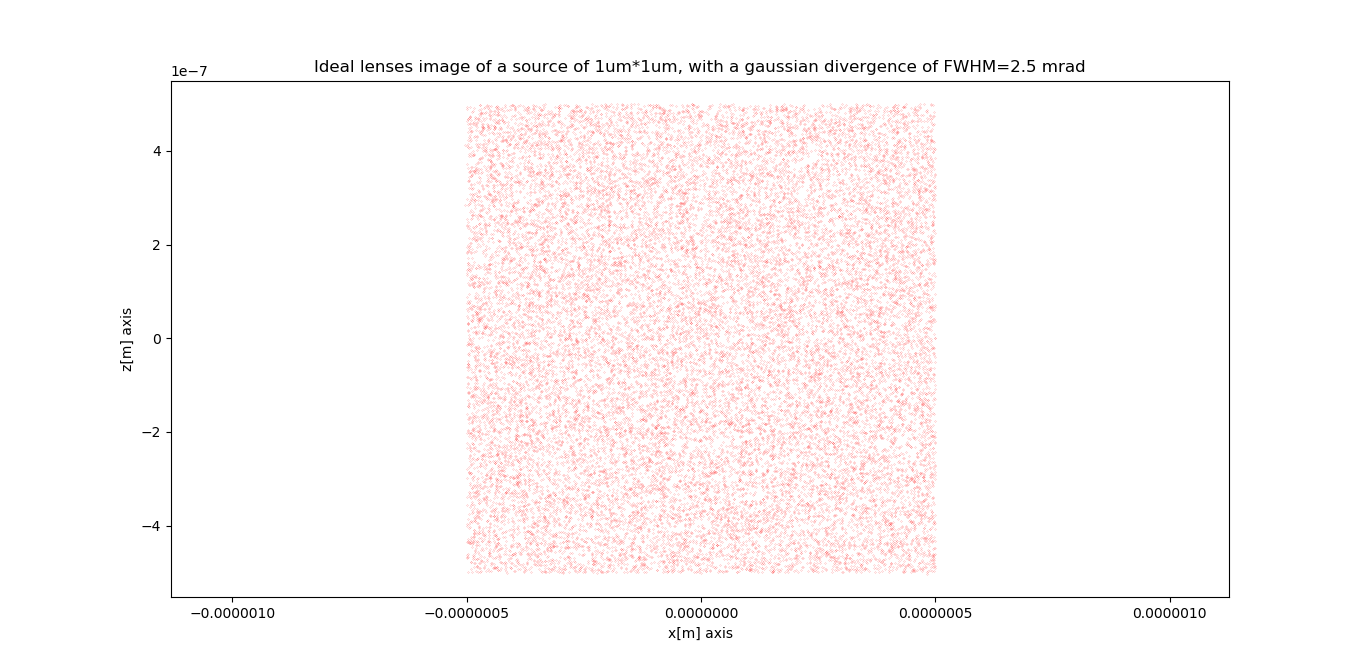
\includegraphics[width=.5\textwidth]{Immagini/Chapter4/IdealLens}}
%
\subfloat[][Initial Beam divergence\label{fig: Ideal Lenses OASYS}]
   {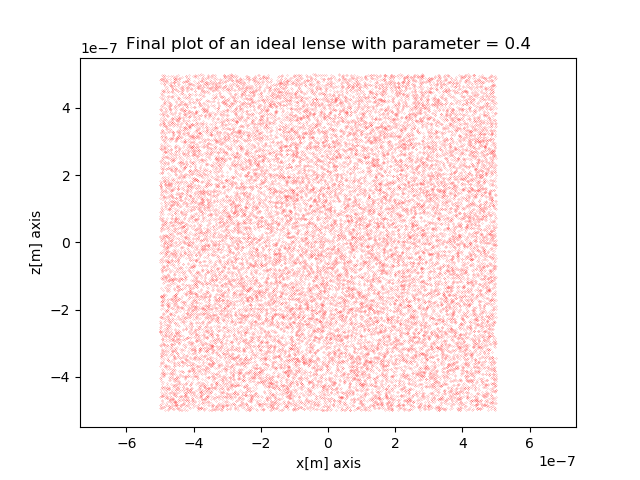
\includegraphics[width=.5\textwidth]{Immagini/Chapter4/IdealLensOASYS}}
%
\caption{Parameter of the source used for the comparison with OASYS}
%
\label{fig: Ideal lense OASYS}
%
\end{figure}
%
\begin{figure}[]
%
\centering
%
\subfloat[][Initial spot size \label{fig: my Paraboloid}]
   {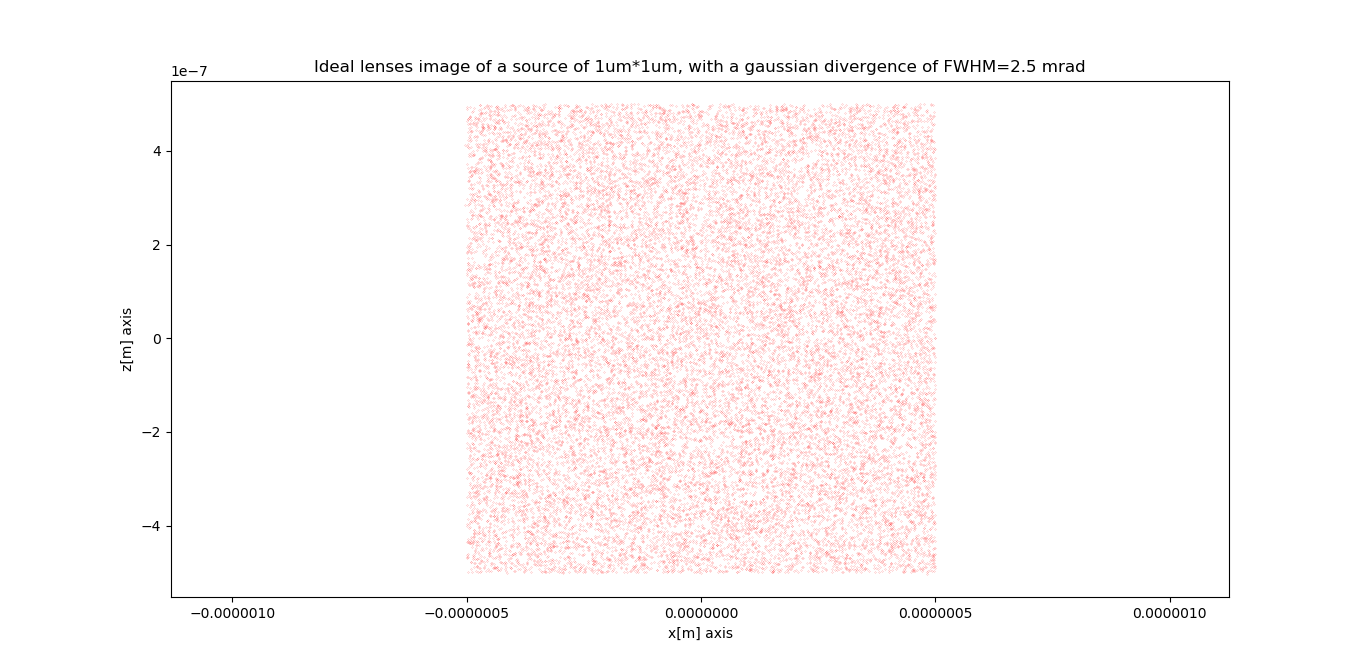
\includegraphics[width=.5\textwidth]{Immagini/Chapter4/IdealLens}}
%
\subfloat[][Initial Beam divergence\label{fig: Paraboloid OASYS}]
   {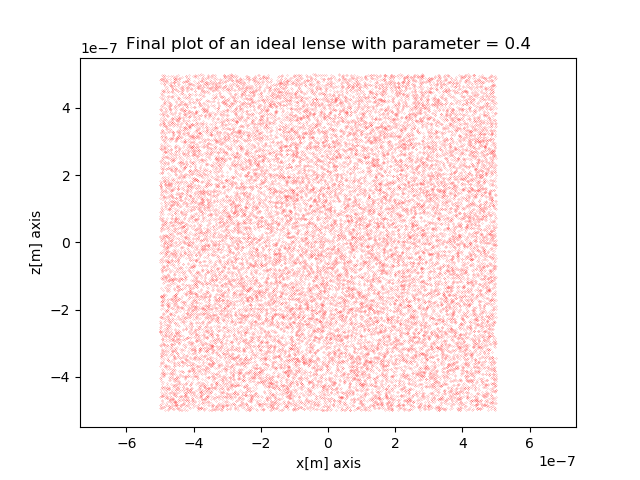
\includegraphics[width=.5\textwidth]{Immagini/Chapter4/IdealLensOASYS}}
%
\caption{Parameter of the source used for the comparison with OASYS}
%
\label{fig: paraboloid OASYS}
%
\end{figure}
%
\begin{figure}[]
%
\subfloat[][Initial spot size \label{fig: my KB }]
   {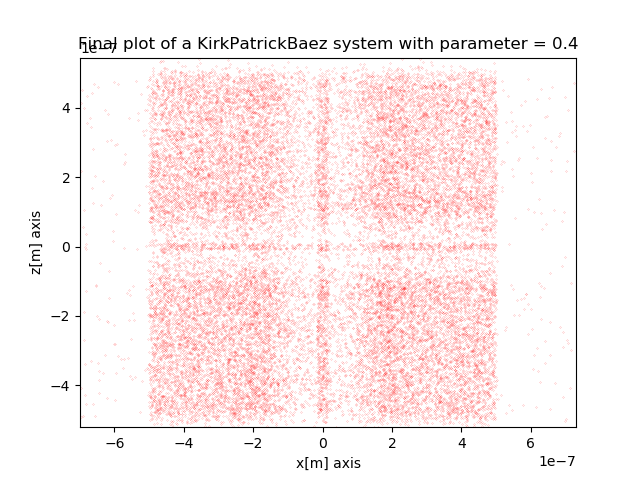
\includegraphics[width=.5\textwidth]{Immagini/Chapter4/KB}}
%
\subfloat[][Initial Beam divergence\label{fig: KB OASYS}]
   {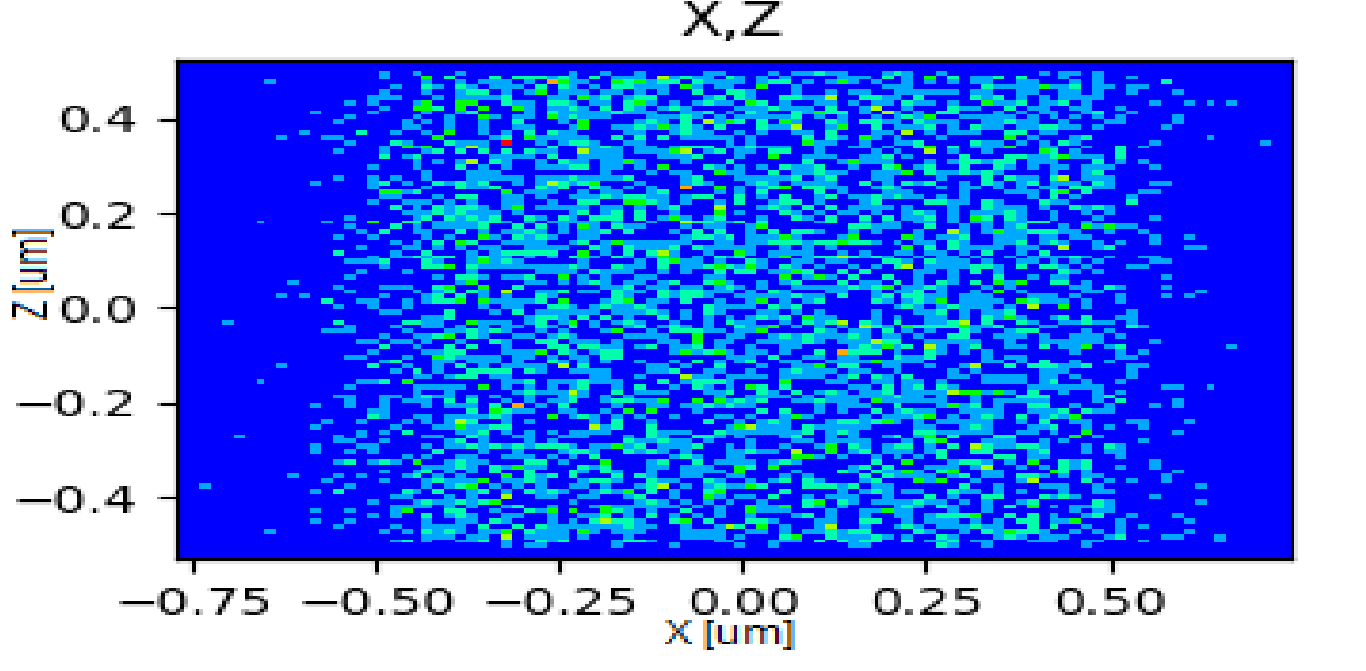
\includegraphics[width=.5\textwidth]{Immagini/Chapter4/KBOASYS}}
%
\caption{Parameter of the source used for the comparison with OASYS}
%
\label{fig: KB system OASYS}
%
\end{figure}
 As it is showed in the figures, the result are pretty similar, with an image that depend on the kind of the system, with the ideal lenses the image is perfect, with KB and paraboloid, the image is similar to the original but degrades with the propagation.
%
\newpage
%
\subsection{Testing with the paper} 
In Figure \ref{fig: PaperMontelSystem} is depicted the Montel system used in the simulation done by the paper in its system of reference. The aim of this system is to collimate a Beam using a Montel with two parabolic mirrors. The source used have a Gaussian dimension with a FWHM of 2.5$\mu $m and a Gaussian divergence of 5$mrad $. The distances, between the source/image plane and the center of the Montel are, respectively,  $\simeq $ 0.26m and 10.06m, moreover, the incidence angle of the Beam is $\theta_g \simeq 2.86^{\circ} $.
%
\begin{figure}[]
	\centering
		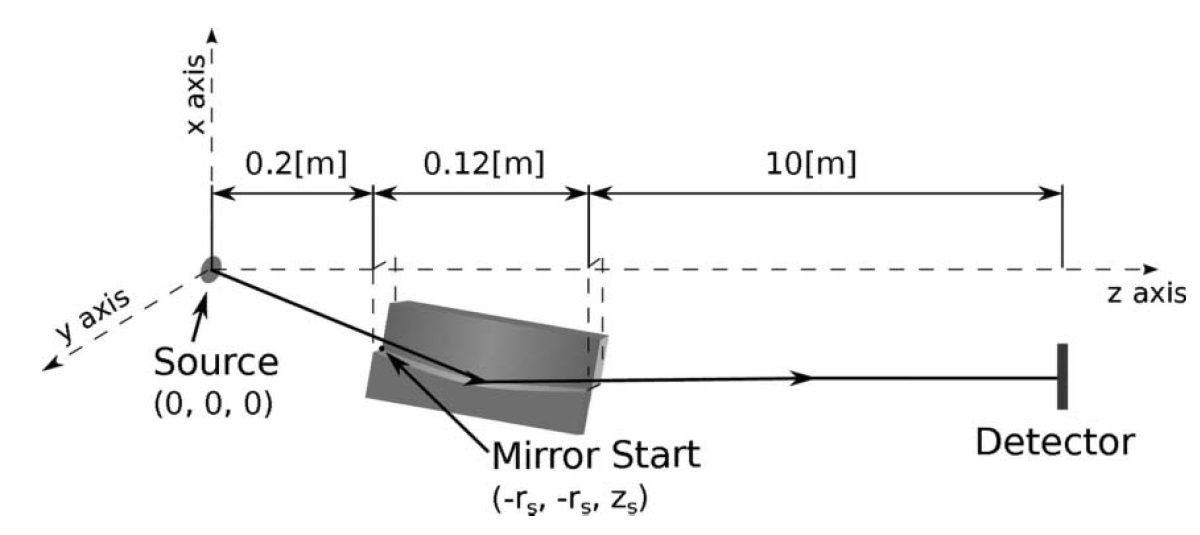
\includegraphics[width=0.8\textwidth]{Immagini/Chapter4/PaperMontelSystem}
		\caption{Illustration of the Montel system used as a collimator in the paper \cite{resta2015nested}}
		\label{fig: PaperMontelSystem}
\end{figure}
%
The result, at the image plane, of the beam size and beam divergence, after the double-reflection of the Montel system, is showed in Figure \ref{fig: My Simulation Comparison}. Where, in Figure \ref{fig: PaperImageShape}, is showed the figure of the beam at the image plane, and, in Figure \ref{fig: PaperImageDivergence}, is showed the divergence. The quantitative values reported on the paper correspond to a Gaussian-like distribution with a spacial FWHM of $\sim $0.7mm, for the spot size, and a FWHM of the Gaussian divergence $\sim $ 0.01 mrad.
\\
Repeating the simulation with my program using the parameter defined in  in the paper \cite{resta2015nested}, are figured out in Figure \ref{fig: My Simulation Comparison}. As it is showed in the Figure \ref{fig: My Simulation Comparison} there are a qualitative good agreement with the two simulation .Also, under a quantitative point of view, there is a good agreement in fact, in my simulation are obtained a value of $\sim $1mm of FWHM of image size, pretty similar to the one of the other simulation, and $\sim $0.01 mrad FWHM of divergence that is equal to the one obtained with the other simulation.
%
\begin{figure}[]
%
\centering
%
\subfloat[][Beam image shape of the paper\label{fig: PaperImageShape}]
   {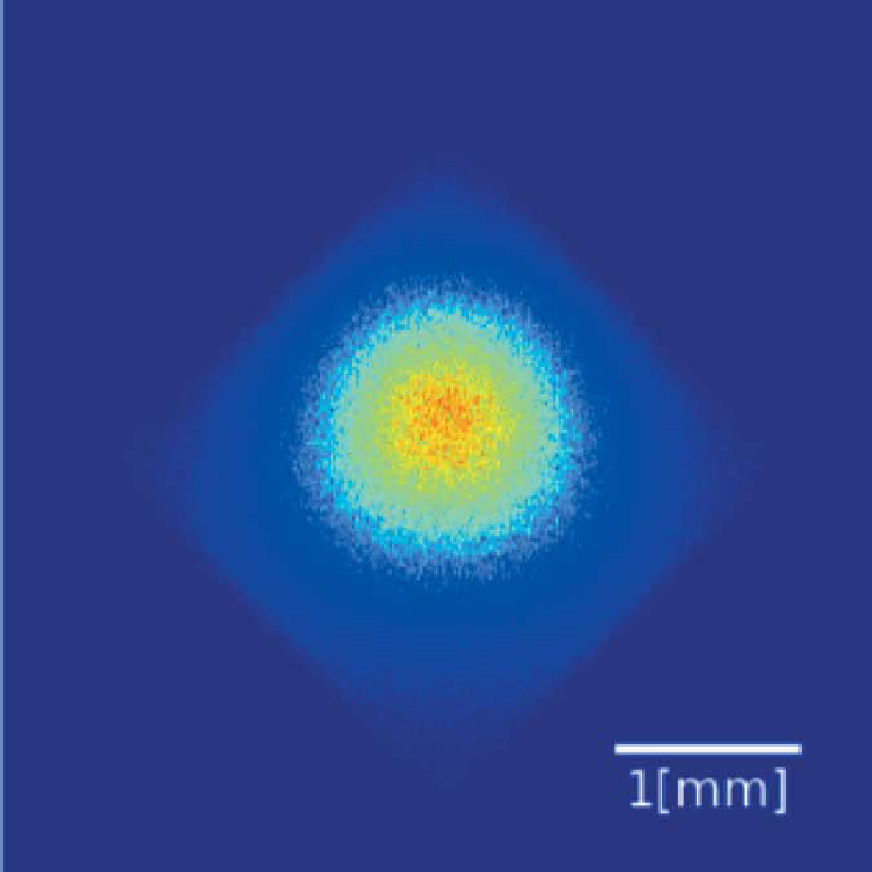
\includegraphics[width=.4\textwidth]{Immagini/Chapter4/PaperSpotMontel}}
%
\subfloat[][Beam image shape of the simulation\label{fig: Image dimension}]
   {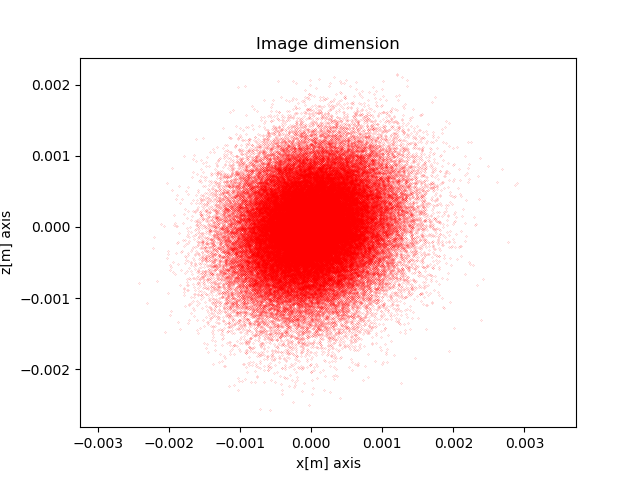
\includegraphics[width=.48\textwidth]{Immagini/Chapter4/ImageDimension}}\quad
%
\subfloat[][Beam image divergence of the paper\label{fig: PaperImageDivergence}]
   {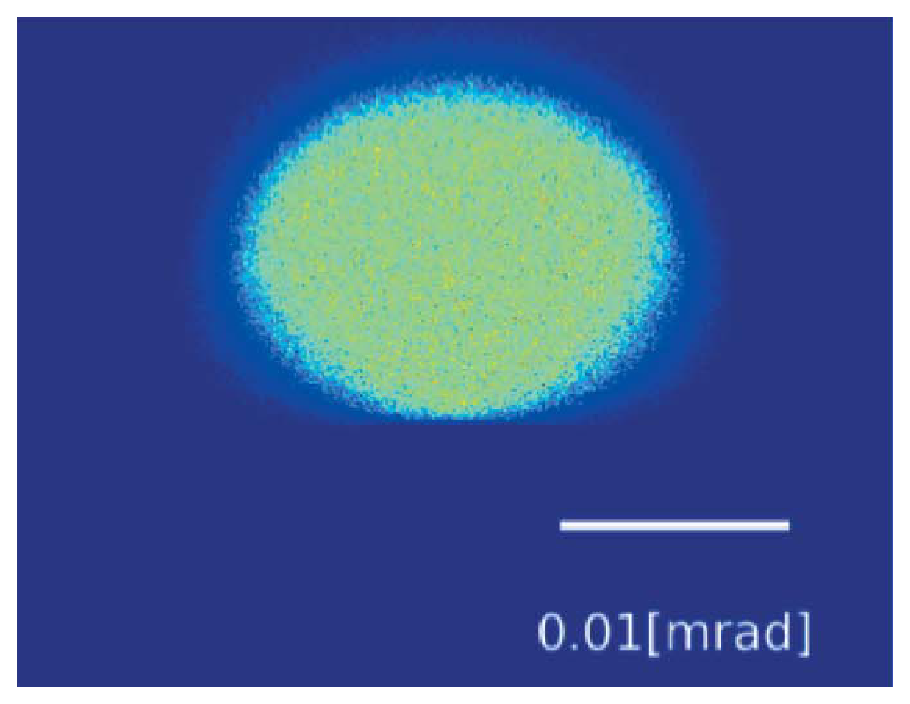
\includegraphics[width=.4\textwidth]{Immagini/Chapter4/PaperDivergenceMontel}}
%
\subfloat[][Beam image divergence of the simulation\label{fig: Divergence dimension}]
   {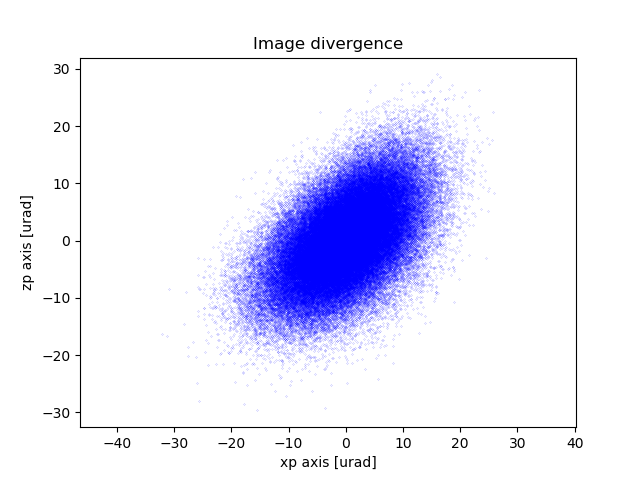
\includegraphics[width=.48\textwidth]{Immagini/Chapter4/DivergenceDimension}}
%
\caption{Results of  the Montel simulations with a source beam with a FWHM spot of 2.5$\mu $m and a Gaussian divergence of 5$mrad $}
%
\label{fig: My Simulation Comparison}
%
\end{figure}
%
\section{Analysis of Montel system}
In this section it is done, using the Montel tools developed, a study of the Montel effect with respect to a Beam, simulating different situation. The first point, to understand that Montel work well, it is simulated the behaviour of a point-wise source with a certain divergence, using a collimating system, and watching what happen to the beam. The  second step is to simulate a collimating beam with a certain source shape geometry and figure out the image plot obtained by a focalizing system in its image plane. What is expected is a point, in the velocity space for the first situation and in the real space for the second simulation, because this is the behaviour of an ideal collimating/focalizing system. For the simulation are used parabolical Montel and an incidence angle of 2$^{\circ} $ (the choice of the angle is arbitrary, that of the paraboic system is because is needed to collimate a beam, also for elliptical system is possible to collimate a beam using one focal distance very big).
\\
In Figure \ref{fig: ideal} are reported the result for the ideal collimating/focalizing cases.
For the collimation system is used a point wise source with a Gaussian divergence of FWHM of 25$\mu $m, \ref{fig: coll.Source}, to the image plane. As it is showed there is a collimation, but not perfect, this effect is one limit of the Montel because the perpendicular geometry is not the ideal one. Moreover, for the focalizing system, it is used a circular source spot having a radius of 1mm, \ref{fig: foc.Source}, with a collimated beam, that show, at the image plane \ref{fig: focalizingImage}, a similar behaviour as for the collimation case, for the same reason.
\begin{figure}[]
%
\centering
%
\subfloat[][Source divergence\label{fig: coll.Source}]
   {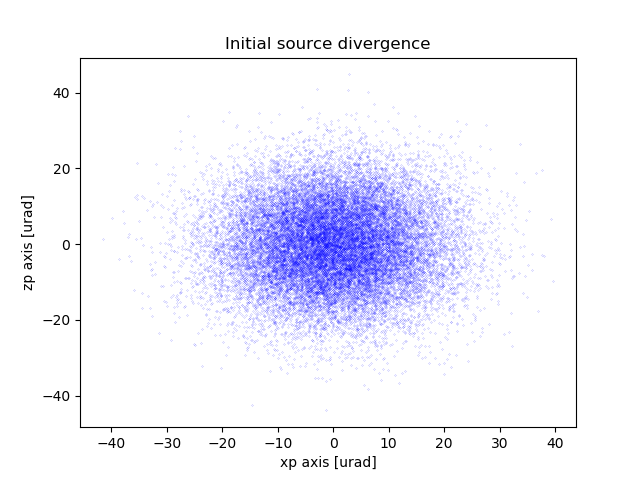
\includegraphics[width=.4\textwidth]{Immagini/Chapter4/CollimationSource}}
%
\subfloat[][Image divergence\label{fig: CollimationImage}]
   {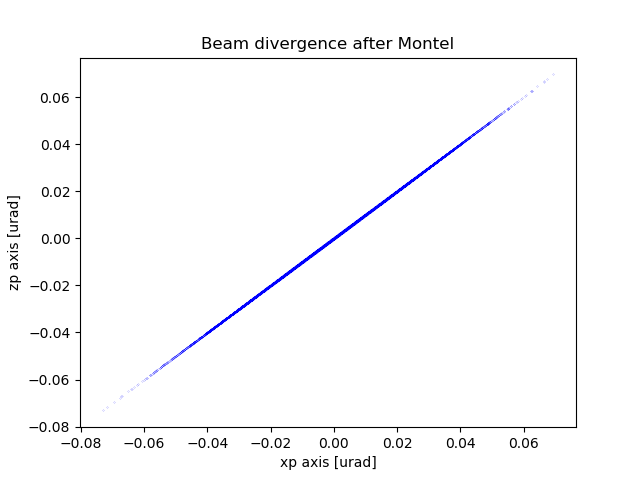
\includegraphics[width=.4\textwidth]{Immagini/Chapter4/CollimationImage}}\quad
%
\subfloat[][Source divergence\label{fig: foc.Source}]
   {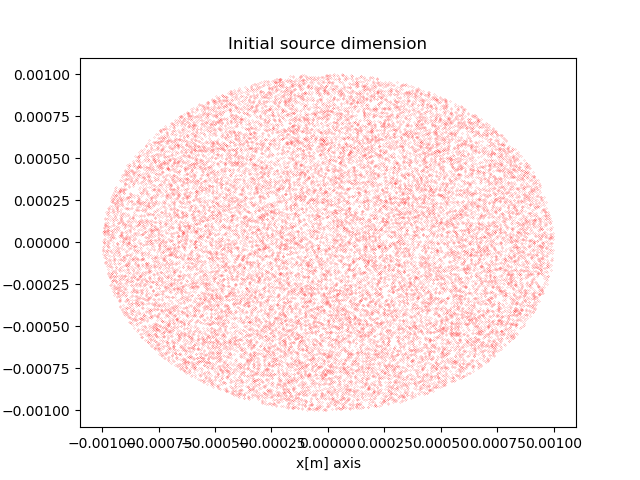
\includegraphics[width=.4\textwidth]{Immagini/Chapter4/FocalizingSource}}
%
\subfloat[][Image divergence\label{fig: focalizingImage}]
   {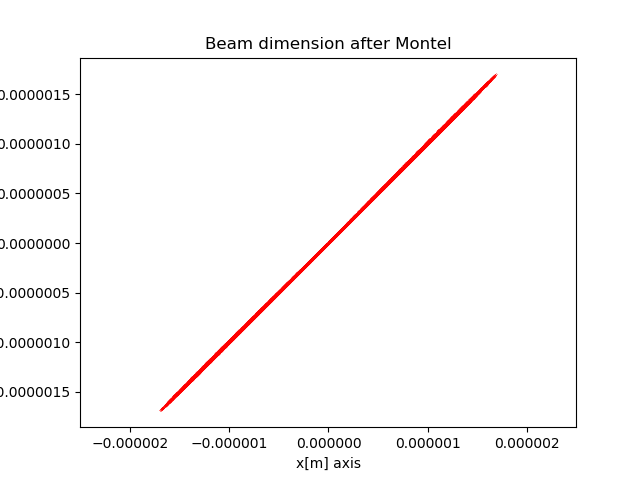
\includegraphics[width=.4\textwidth]{Immagini/Chapter4/FocalizingImage}}
%
\caption{Ideal system}
%
\label{fig: ideal}
%
\end{figure}
%
Another interested point to show is the footprint on the two mirror that are represented in Figure \ref{fig: footprint}. It is possible to note that the area hit by the beam have a greater component on the y direction (due to the grazing incidence), than in the other direction. In this particular case the x-lenght of the xy-mirror, and the z-lenght of the zy-mirror, is very small (at the order of 20$\mu $m) with respect to the y-lenght that is $\sim $20mm. These calculatione are done for a very small Gaussian spot with a FWHM of 1$\mu $m and a narrow divergence of FWHM equal to 25$\mu $rad.
\begin{figure}[]
%
\centering
%
\subfloat[][Footprint on oe1\label{fig: footprint_oe1}]
   {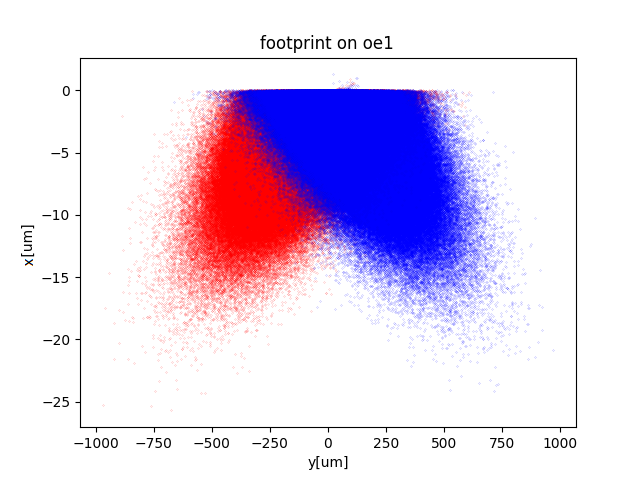
\includegraphics[width=.4\textwidth]{Immagini/Chapter4/footprint_oe1}}
%
\subfloat[][Footprint on oe2\label{fig: footprint_oe2}]
   {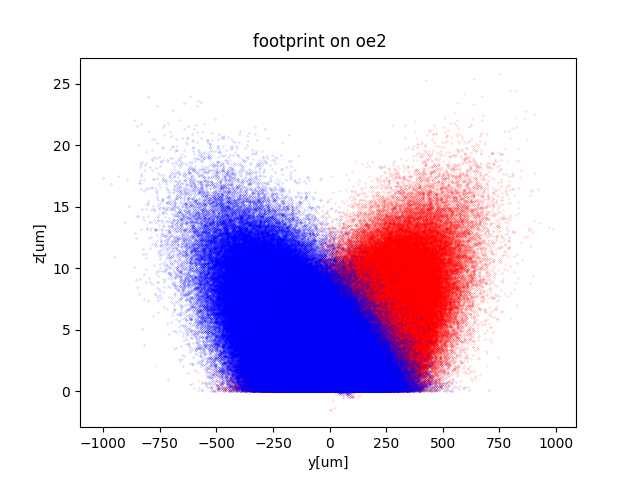
\includegraphics[width=.4\textwidth]{Immagini/Chapter4/footprint_oe2}}\quad
%
\caption{Footprint, on the xy-mirror (\ref{fig: footprint_oe1}) and on zy-mirror (\ref{fig: footprint_oe2}). The red dots are those rays that hit before xy-mirror and after zy-mirror, the blue ones hit first xy-mirror and after zy-mirror.}
%
\label{fig: footprint}
%
\end{figure}
Up to know the dimension of the Montel were not considered, the Montel is set to have infinite dimension in all the direction. This approach hold in the case of a small source and a narrow profile divergence, otherwise, for example of an isotropic source that can be modelled with a very big divergence the situation change. In this section, it is used a Beam source with a square shape with a side of 1mm, with a Gaussian profile divergence of FWHM=1mrad in order to show what happen to the Montel  where it is covered over all its surface. The focalizing parabolic Montel parameter are:
\begin{itemize}
\item object  distance: 1m
\item image distance: 3m
\item incidence angle: $2^{\circ} $
\item length of the Monte: 0.1m
\item width of the Montel: 20cm
\end{itemize}
%
\begin{figure}[]
%
\centering
%
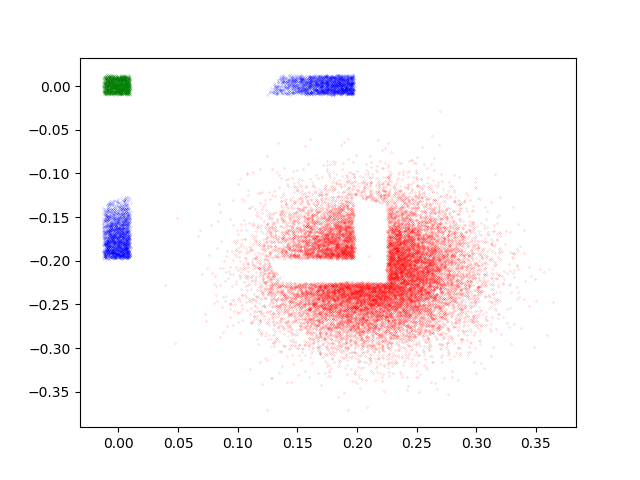
\includegraphics[width=.6\textwidth]{Immagini/Chapter4/BigSourceMontel}
%
\caption{Illumination at the image plane of the different Beam (red dots correspond to np-reflected rays, blue dot to one-reflected rays, green dots to two-reflected rays).}
%
\label{fig:BigSourceMontel}
%
\end{figure}
%
Figure \ref{fig:BigSourceMontel}, show thee image plane of the Montel defined above. This plot show 4 figure, the biggest one, represented by the red dots, correspond to the rays that reach the image plane without touch the Montel, the rays coloured in blue, are those which are subject to only one reflection that are positioned in different part of the image plane depending which mirror meet, those that hit the xy-mirror correspond to the beam elongated along z, the zy-mirror correspond to the beam elongate along x. At the end, the green dots, are the rays that do both reflection and are centred to the center of the image plane by definition of it. 
\subsection{Alignment}
Alignment of a beam is important for experimental use so, this section studies the behaviour of a beam when the beam is not perfectly align, in order to understand the behaviour of the beam in the different cases and act consequently. 
\\
The parameter that are changed are :
\begin{enumerate}
	\item orthogonality
	\item incidence angle
	\item point of incidence
\end{enumerate}
Using a focusing parabolic Montel system with a source of square shape having a side of 1$\mu $m, and a Gaussian divergence with FWHM of 25$\mu $m

\subsection{Alignment: Orthogonality}
In this section is it done an orthogonality studies of the Montel system, it is studied the behaviour of a beam, using a source parameter defined before. Figure \ref{fig:HistogramFitted} presents the interesting histogram versus the horizontal angle $x^{'} $ when the angle between the mirrors change ($\alpha = 90^{\circ} + \Delta $). It can be noted a improvement of the collimation of the beam changing the angle in the case of closer mirrors ($\Delta = -0.004^{\circ} $).
\\
Figure show the trend of the FWHM of the $x^{'} $ changing the angle $\Delta $, it is possible to note a minimum for negative angle (this  situation correspond to the indigo line) after that the situation become worse. Moreover, the behaviour of the FWHM is not symmetric with respect to $0^{\circ} $, in case of negative angle deviation the situation improve for small range of deviation angle, after that, the trend get worse, on the opposite way, the situation get worse increasing the positive deviation angle. 
%
%\begin{figure}[]
%
%\centering
%
%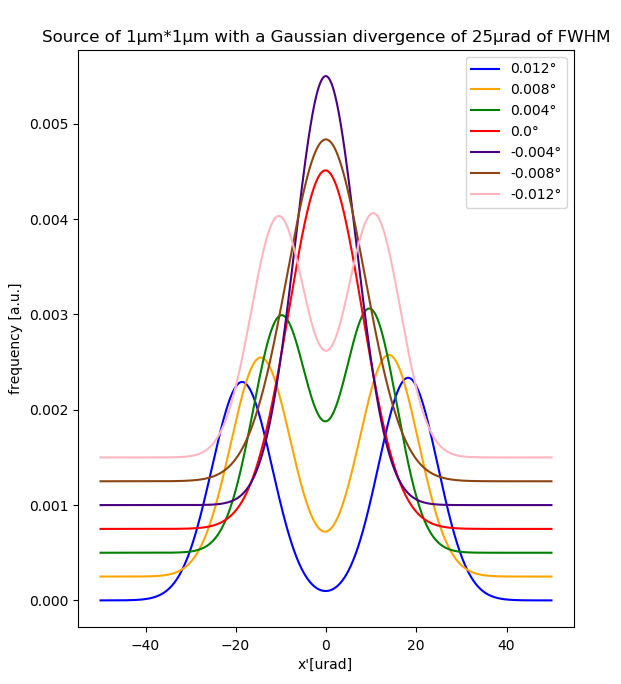
\includegraphics[width=.6\textwidth]{Immagini/Chapter4/HistogramFitted}
%
%\caption{x' values after the Montel system}
%
%\label{fig:HistogramFitted}
%
%\end{figure}
%%%%%%%%%%%%%%%%
\begin{figure}[]
%
\centering
%
\subfloat[][Real histogram\label{fig:HistogramFitted2}]
   {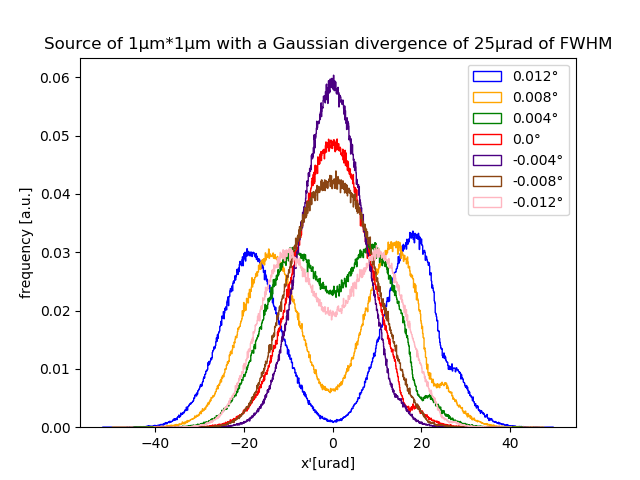
\includegraphics[width=0.6\textwidth]{Immagini/Chapter4/Histogram}}\quad
%
\subfloat[][Fitted Histogram\label{fig:HistogramFitted}]
   {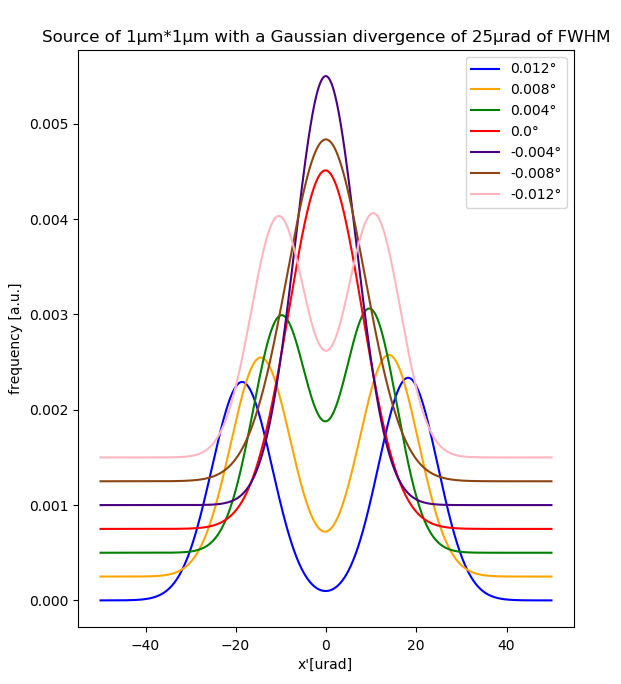
\includegraphics[width=.6\textwidth]{Immagini/Chapter4/HistogramFitted}}
%
\caption{Histogram of x' after Montel}
%
\label{fig: incidence angle}
%
\end{figure}
%%%%%
\begin{figure}
%
\centering
%
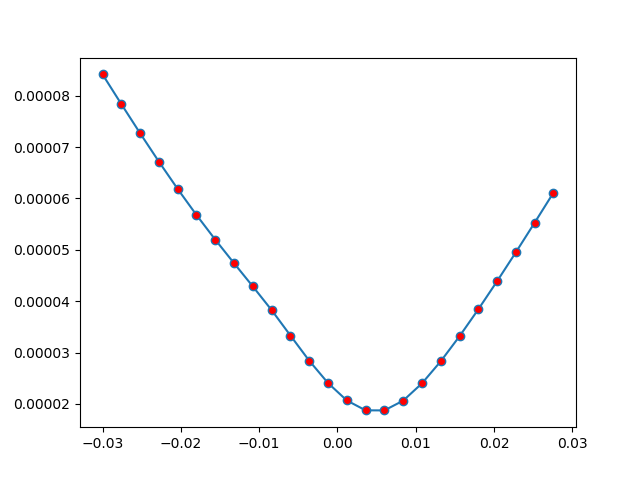
\includegraphics[width=.6\textwidth]{Immagini/Chapter4/FWHMChangingOrt}
%
\caption{FWHM of x' after the Montel changing the orthogonality}
%
\label{fig:FWHM changing orthogonality}
%
\end{figure}
\subsection{Alignment: Incidence angle}
To understand the behaviour of a non aligned beam it is simulated the situation of a beam that arrive at the Montel system with the wrong angle. In this particular case the system is defined as follow: incidence angle of $3^{\circ} $, square spot of 100$\mu $ $m^{2} $, Gaussian divergence with FWHM of 25$\mu $rad. Figure
\begin{figure}[]
%
\centering
%
\subfloat[][fwhm\label{fig: footprint_oe1}]
   {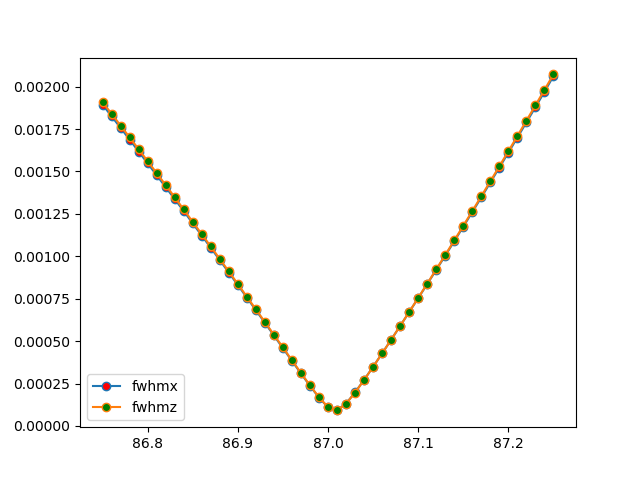
\includegraphics[width=.4\textwidth]{Immagini/Chapter4/IncidenceAngle}}
%
\subfloat[][splitting of fwhm\label{fig: footprint_oe2}]
   {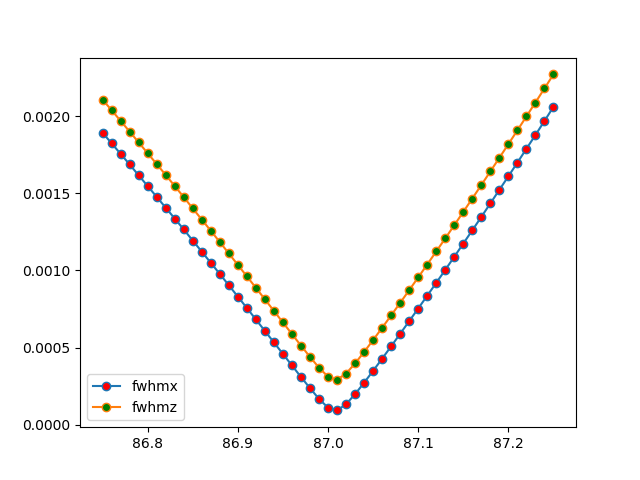
\includegraphics[width=.4\textwidth]{Immagini/Chapter4/IncidenceAngle2}}\quad
%
\caption{Incidence angle}
%
\label{fig: incidence angle}
%
\end{figure}
\subsection{Alignment: point of incidence}
Another way that can be studied to align correctly a beam, is to study the behaviour of a non centred beam with respect to the center of the Montel system. In this section is reported the behaviour about the change of FWHM of both $x^{'} $ and $z^{'} $ following different path. Figure \ref{fig: path} show the different path followed to simulate the non-centred beam that are named:
\begin{enumerate}
	\item Y
	\item XZ
	\item XYZ1
	\item XZY2
\end{enumerate}

\begin{figure}[]
%
\centering
%
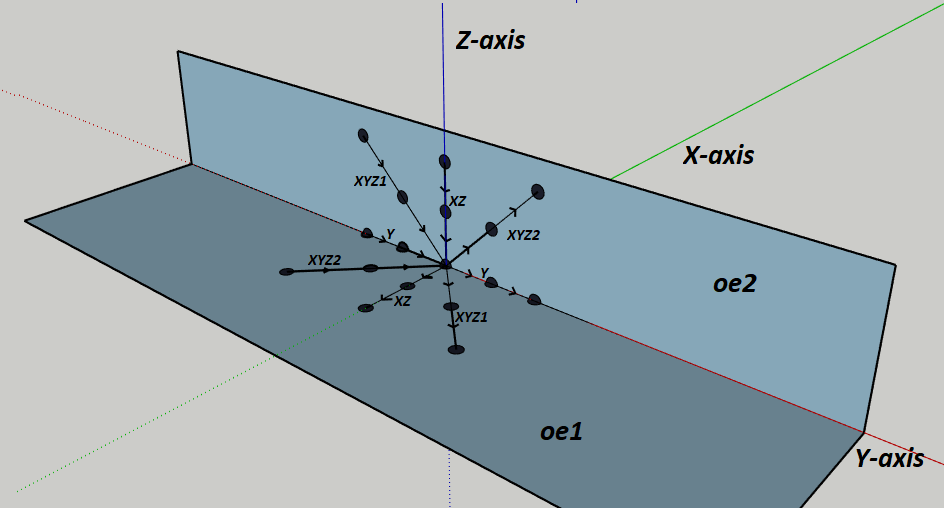
\includegraphics[width=1.\textwidth]{Immagini/Chapter4/Cattura2}
%
\caption{Different path for simulate the non-centred beam}
%
\label{fig: path}
%
\end{figure}

Figure \ref{fig: reuslt diff. path} show the behaviour of the two FWHM of the beam changing the incidence point of the beam moving the different paths. This point is defined with respect to the center of the Montel system that correspond to the origin (0, 0, 0). In Figure \ref{fig: Y path}, the incidence point move along y-axis, start from the point (0, 1.5mm, 0) and arriving to the point (0, -1.5mm, 0), and show, more or less, a flat behaviour of the FWHM. Figure \ref{fig: XZ path} start from the point (0, 0, 0.15mm) and arrive to (-0.15mm, 0, 0) and have specular behaviour for the two FWHM, there is a minimum of the two FWHM near the origin point, moving on the oe1 worse the FWHM of $z^{'} $ and maintain the other constant, on the contrary, moving on the oe2 the situation is reversed, in this case the FWHM of $x^{'} $ get worse, maintaining constant the one of $z^{'} $. Figure \ref{fig: XYZ1 path} start from (0, 1.5mm, 0.15mm) and arrive to (-0.15mm, -1.5mm, 0) and Figure \ref{fig: XYZ2 path} start from (-0.15mm, 1.5mm, 0) and arrive to (0., -1.5mm, 0.15mm). The behaviour of this last two path are similar to that of \ref{fig: XZ path}, this is reasonable, because the motion along y-axis does not influence the FWHM because of the definition of the cylindrical mirror, that in any point along the y direction have the same geometry.
%
%
\begin{figure}[]
%
\centering
%
\subfloat[][Y path\label{fig: Y path}]
   {\includegraphics[width=.4\textwidth]{Immagini/Chapter4/Ypath}}
%
\subfloat[][XZ path\label{fig: XZ path}]
   {\includegraphics[width=.4\textwidth]{Immagini/Chapter4/XZpath}}\quad
%
\subfloat[][XYZ1 path\label{fig: XYZ1 path}]
   {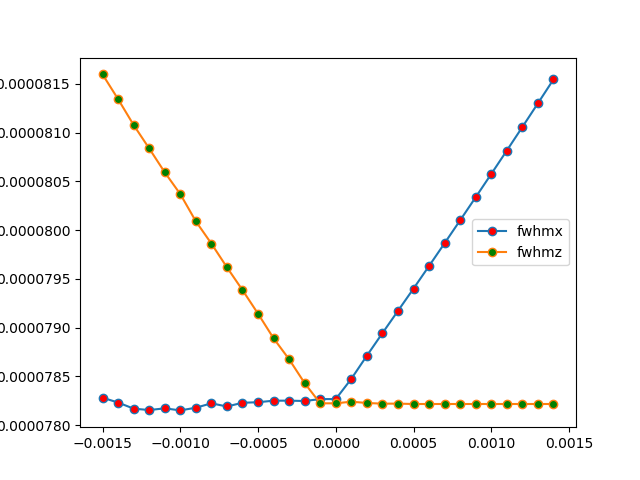
\includegraphics[width=.4\textwidth]{Immagini/Chapter4/XYZ1Path}}
%
\subfloat[][XYZ2 path\label{fig: XYZ2 path}]
   {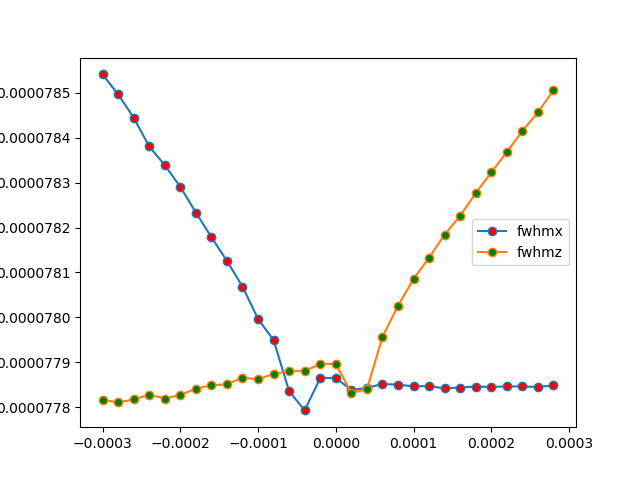
\includegraphics[width=.4\textwidth]{Immagini/Chapter4/XYZ2Path}}
\caption{Resuts of the Montel system of a source beam with a FWHM spot of 2.5$\mu $m and a Gaussian divergence of 5$mrad $}
%
\label{fig: reuslt diff. path}
%
\end{figure}
In Figure \ref{fig: 2nd reuslt diff. path} it is show the intensity profile of the two-reflection beam after the Montel, calculated as the number of the rays in the two-reflection beam with respect to the initial number of rays. The source used, in this case, correspond to a big spot of a square geometry with an area of $1mm^2 $, and a large Gaussian divergence with a FWHM of 10mrad. The Montel used is a parabolic localizing system having e an object distance of 1m, an image distance of 3m, an incidence angle of $2^{\circ} $ and a finite dimension, with a length of 20cm and a width of 2cm.
The different path move along these points; ymax=50cm, ymin=-50cm, xmin=-2cm, xmax=0, zmax=2cm, zmin=0
\\
The plots in Figure \ref{fig: 2nd reuslt diff. path}, are interesting, because represents the intensity of the "green" Beam in Figure \ref{fig:BigSourceMontel}, that can be directly measured and so, it is possible to realted the centring of the Beam calculating the intensity of this Beam.
%
\begin{figure}[]
%
\centering
%
\subfloat[][Y path\label{fig: Y path}]
   {\includegraphics[width=.4\textwidth]{Immagini/Chapter4/Ypath_2}}
%
\subfloat[][XZ path\label{fig: XZ path}]
   {\includegraphics[width=.4\textwidth]{Immagini/Chapter4/XZpath_2}}\quad
%
\subfloat[][XYZ1 path\label{fig: XYZ1 path}]
   {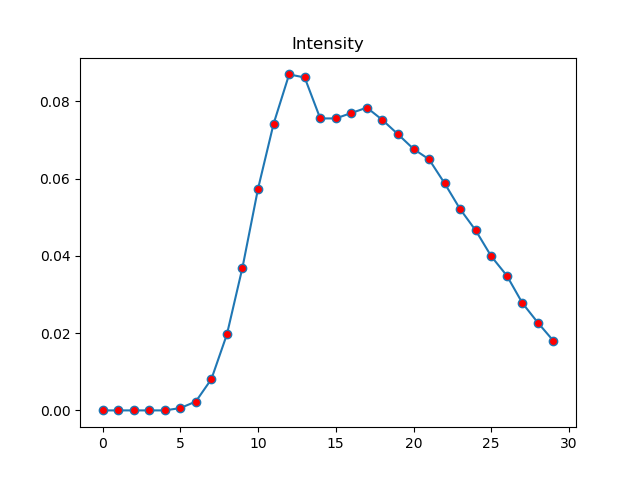
\includegraphics[width=.4\textwidth]{Immagini/Chapter4/XYZ1Path_2}}
%
\subfloat[][XYZ2 path\label{fig: XYZ2 path}]
   {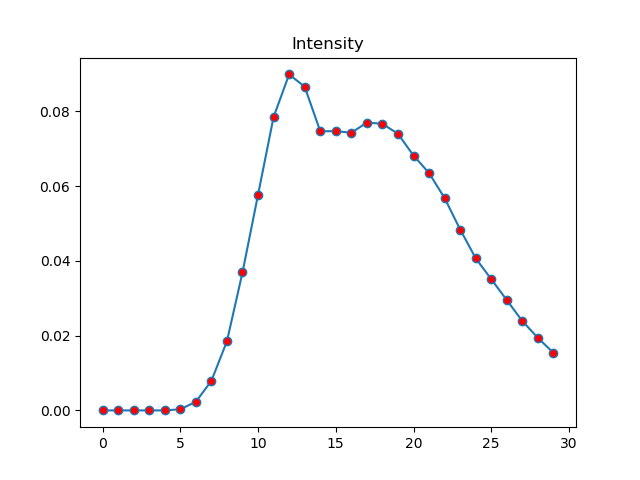
\includegraphics[width=.4\textwidth]{Immagini/Chapter4/XYZ2Path_2}}
\caption{Resuts of the Montel system of a source beam with a FWHM spot of 2.5$\mu $m and a Gaussian divergence of 5$mrad $}
%
\label{fig: 2nd reuslt diff. path}
%
\end{figure}